%%%%%%%%%%%%%%%%%%%%%%%%%%%%%%%%%%%%%%%%%
% Beamer Presentation
% LaTeX Template
% Version 1.0 (10/11/12)
%
% This template has been downloaded from:
% http://www.LaTeXTemplates.com
%
% License:
% CC BY-NC-SA 3.0 (http://creativecommons.org/licenses/by-nc-sa/3.0/)
%
%%%%%%%%%%%%%%%%%%%%%%%%%%%%%%%%%%%%%%%%%

%----------------------------------------------------------------------------------------
%	PACKAGES AND THEMES
%----------------------------------------------------------------------------------------

\documentclass{beamer}

\mode<presentation> {

% The Beamer class comes with a number of default slide themes
% which change the colors and layouts of slides. Below this is a list
% of all the themes, uncomment each in turn to see what they look like.

%\usetheme{default}
%\usetheme{AnnArbor}
%\usetheme{Antibes}
%\usetheme{Bergen}
%\usetheme{Berkeley}
%\usetheme{Berlin}
%\usetheme{Boadilla}
%\usetheme{CambridgeUS}
%\usetheme{Copenhagen}
%\usetheme{Darmstadt}
%\usetheme{Dresden}
%\usetheme{Frankfurt}
%\usetheme{Goettingen}
%\usetheme{Hannover}
%\usetheme{Ilmenau}
%\usetheme{JuanLesPins}
%\usetheme{Luebeck}
\usetheme{Madrid}
%\usetheme{Malmoe}
%\usetheme{Marburg}
%\usetheme{Montpellier}
%\usetheme{PaloAlto}
%\usetheme{Pittsburgh}
%\usetheme{Rochester}
%\usetheme{Singapore}
%\usetheme{Szeged}
%\usetheme{Warsaw}

% As well as themes, the Beamer class has a number of color themes
% for any slide theme. Uncomment each of these in turn to see how it
% changes the colors of your current slide theme.

%\usecolortheme{albatross}
%\usecolortheme{beaver}
%\usecolortheme{beetle}
%\usecolortheme{crane}
%\usecolortheme{dolphin}
%\usecolortheme{dove}
%\usecolortheme{fly}
%\usecolortheme{lily}
%\usecolortheme{orchid}
%\usecolortheme{rose}
%\usecolortheme{seagull}
%\usecolortheme{seahorse}
%\usecolortheme{whale}
%\usecolortheme{wolverine}

%\setbeamertemplate{footline} % To remove the footer line in all slides uncomment this line
%\setbeamertemplate{footline}[page number] % To replace the footer line in all slides with a simple slide count uncomment this line

%\setbeamertemplate{navigation symbols}{} % To remove the navigation symbols from the bottom of all slides uncomment this line
}

\usepackage{graphicx} % Allows including images
\DeclareGraphicsExtensions{.pdf,.png,.jpg}
\usepackage{booktabs} % Allows the use of \toprule, \midrule and \bottomrule in tables
\usepackage[skip = 2pt, font=scriptsize]{caption}
\usepackage{subfigure}

%----------------------------------------------------------------------------------------
%	TITLE PAGE
%----------------------------------------------------------------------------------------

\title[Antineutrons]{Antineutrons Produced from Antiprotons in Charge-Exchange Collisions} % The short title appears at the bottom of every slide, the full title is only on the title page

\author{Oliver Dahme} % Your name
\institute[UZH] % Your institution as it will appear on the bottom of every slide, may be shorthand to save space
{
University of Zurich \\ % Your institution for the title page
\medskip
\textit{o.dahme@cern.ch} % Your email address
}
\date{\today} % Date, can be changed to a custom date

\begin{document}

\begin{frame}
\titlepage % Print the title page as the first slide
\end{frame}

\begin{frame}
\frametitle{Overview} % Table of contents slide, comment this block out to remove it
\tableofcontents % Throughout your presentation, if you choose to use \section{} and \subsection{} commands, these will automatically be printed on this slide as an overview of your presentation
\end{frame}

%----------------------------------------------------------------------------------------
%	PRESENTATION SLIDES
%----------------------------------------------------------------------------------------

%------------------------------------------------
\section{Introduction} % Sections can be created in order to organize your presentation into discrete blocks, all sections and subsections are automatically printed in the table of contents as an overview of the talk
%------------------------------------------------

\begin{frame}
\frametitle{Idea}
\begin{itemize}
  \item Antiprotons where already known
  \item Are there also Antineutrons?
  \item What happens if C conjugation is applied on neutral particles?
  \item If they can be produced from Antiprotons, a large flux (300-600) is required
\end{itemize}
% When Antiprotons where discoverd, it raised the question what would happen if
% the charge conjugation is applied on neutral particles like the Neutron. \\
% The purpose of this experiment was to to detect the annihilation of antineutrons
% produced by charge exchange of antiprotons. \\
% Since the yield of antineutrons was expected to be low a large flux of antiprotons (300-600) was required.
\end{frame}

%------------------------------------------------

\begin{frame}
\frametitle{Experimental Set-Up}
\begin{figure}
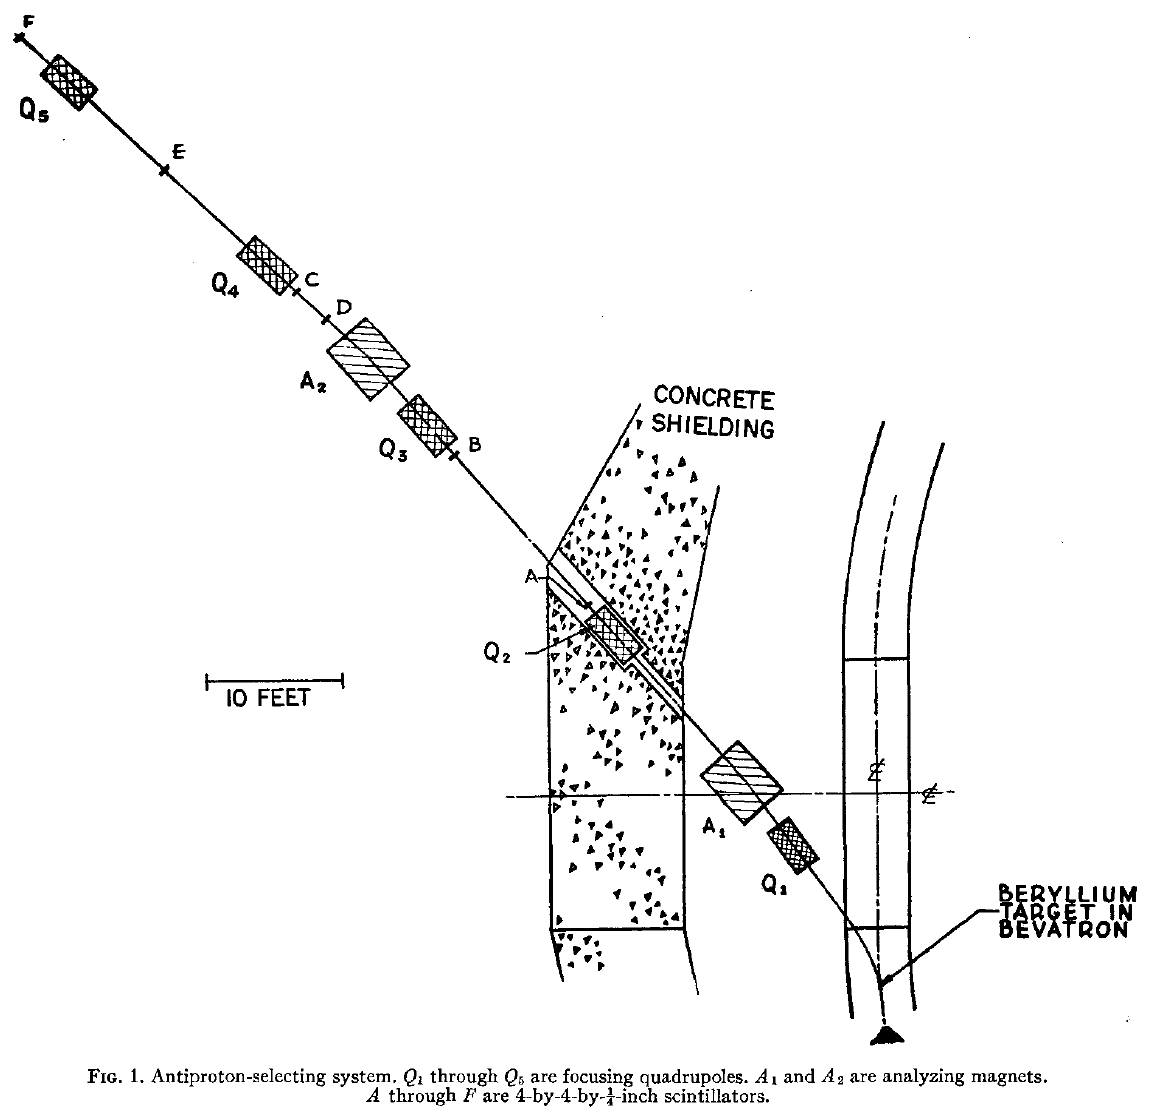
\includegraphics[width=0.65\textwidth]{experiment}
\end{figure}
\end{frame}

%------------------------------------------------

\begin{frame}
\frametitle{Experimantal Set-Up}
\begin{itemize}
  \item Protons + Beryllium = Antiprotons + ...
  \item scintillators detect them and other charge particles (A-F)
  \item heart of the experiment: A lead glas Cherenkov detector (C)
  \item in a second run the Cherenkov detector was replaced by a large Scintillator
\end{itemize}
% To produce Antiprotons, Protons from the Bevatron where shot on to a Beryllium target. \\
% These are then focused by magnets. To deteced them several scintillators are placed along the path. \\
% The heart of the experiment is the Chernkov Counter in C it uses lead glas as Cherenkov emitter. \\
% It is used to deteced neutral Mesons and ordinary neutrons through Chernkov light which has low energy. \\
% But the Photomultiplier are also capable to deteced the Annihialtion light of antineutrons interacting with the
% lead glas inside the detector which has much higher energy than the Cherenkov light of neutral particles. \\
% Therefore is is able to deteced antineutrons. \\
% After the experiment the Cherenkov Detector was replaced by a large scintillator.
\end{frame}

\begin{frame}
\frametitle{lead glas Cherenkov detecor}
\begin{figure}
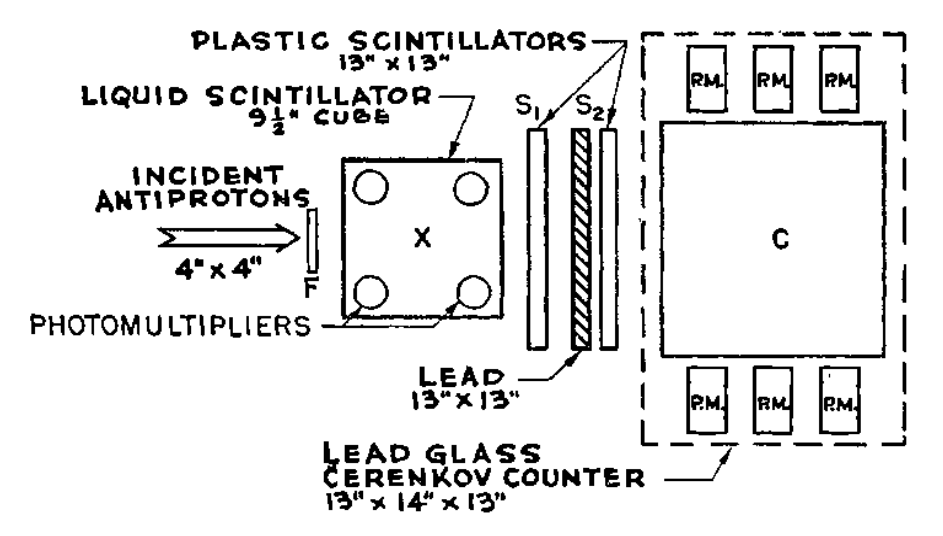
\includegraphics[width=0.45\textwidth]{detector}
\end{figure}

\begin{itemize}
  \item Antiprotons collide with the lead plate $\Rightarrow$ Antineutrons are created
  \item Antineutrons annihilate in the lead glas
  \item Light from annihilation gets deteced
\end{itemize}
\end{frame}


\section{Results}
%------------------------------------------------

\begin{frame}
\frametitle{results with Cherenkov detector}
\begin{figure}
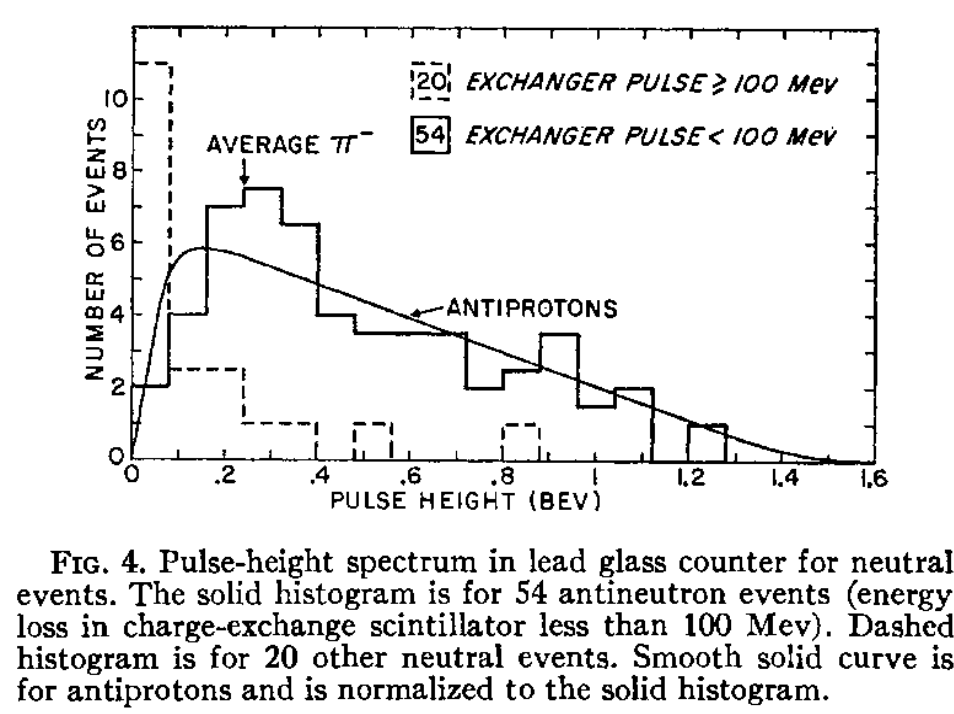
\includegraphics[width=0.45\textwidth]{result1}
\end{figure}
\begin{itemize}
  \item Energy scale comes from relating puls height and shape to $\pi$-mesons
  \item Smooth curve provides the annihilation pulse-height distribution of antiprotons
  \item Histogram is the measured data
  \item since it is similar to the one of antiprotons, antineutrons exist
\end{itemize}
% The energy scale is obtained by realting the puls height and shape to $\pi$-mesons
% going through the glas which have ionization energy of 240 MeV. \\
% The smooth curve provides the Annihilation pulse-height distribution, it is optained
% by sending antiprotons in the detector without the lead glass shielding. \\
% As one can see the histogram provides a similar distribution even with the shielding
% which confirms that the events are antineutrons.
\end{frame}

%------------------------------------------------
% Sections can be created in order to organize your presentation into discrete blocks, all sections and subsections are automatically printed in the table of contents as an overview of the talk
%------------------------------------------------

\begin{frame}
\frametitle{results with large scintillator}
\begin{figure}
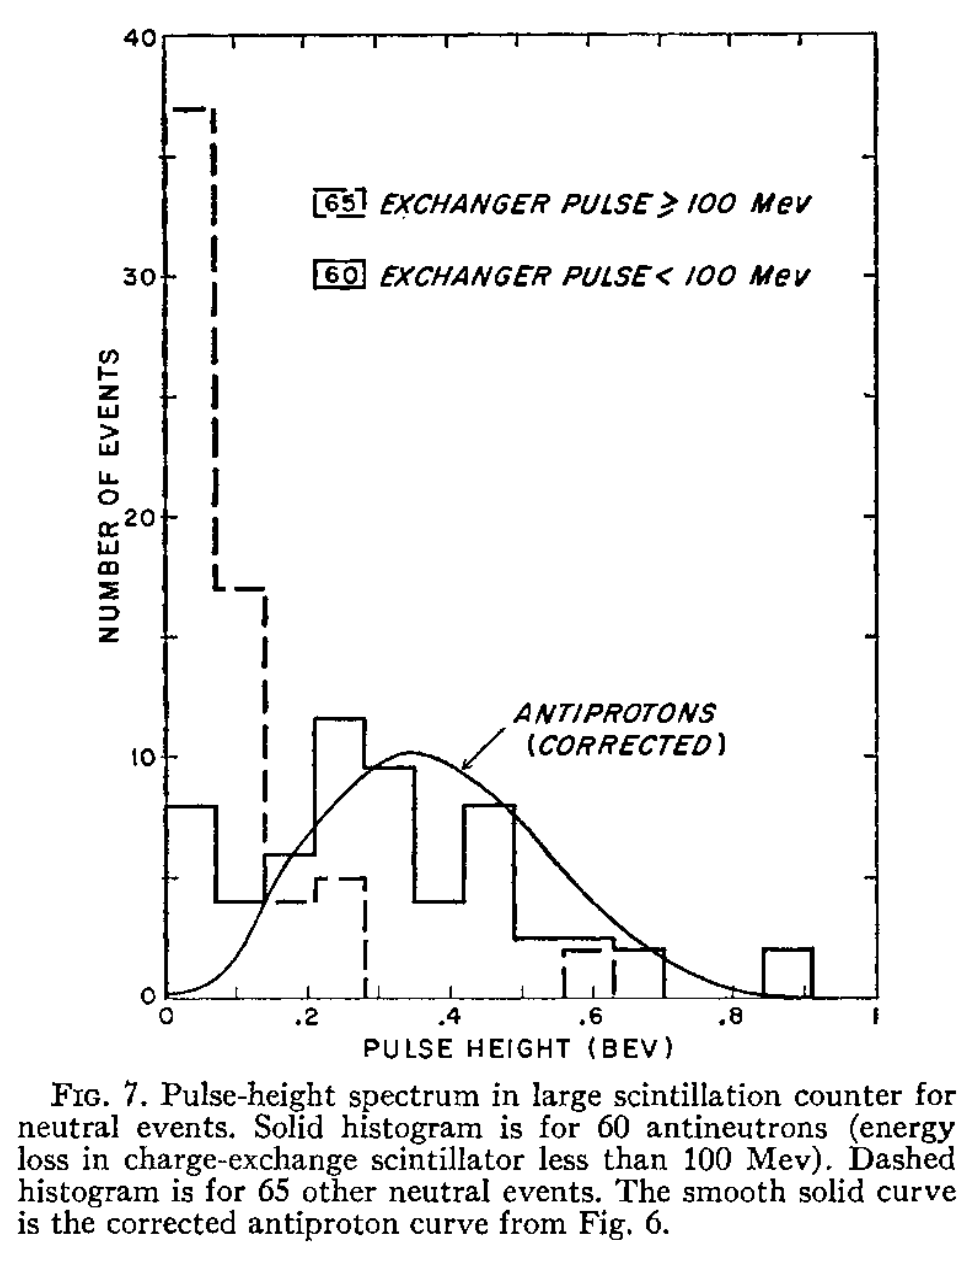
\includegraphics[width=0.3\textwidth]{result2}
\end{figure}
\begin{itemize}
  \item large scintillator provides a similar pulse height distribution
  \item it also confirms the existance of antineutrons
\end{itemize}
% Also for the large scintillator a pulse-height distribution similar to the one
% of antiprotons was produced. It therfore also confirms the existance of antineutrons.
\end{frame}

%------------------------------------------------
\begin{frame}
\frametitle{Comparison of results}
\begin{itemize}
  \item In the lead glas detector $0.0030 \pm 0.0005$ antineutrons per antiproton had been detected.
  \item For the large scintilator $0.0028 \pm 0.0005$ antineutrons per antiproton had been detected.
  \item $\Rightarrow$ The efficiency is nearly equal.
\end{itemize}
\end{frame}

%------------------------------------------------

\section{today}
\label{sec:today}


\begin{frame}
\frametitle{today}
\begin{figure}
  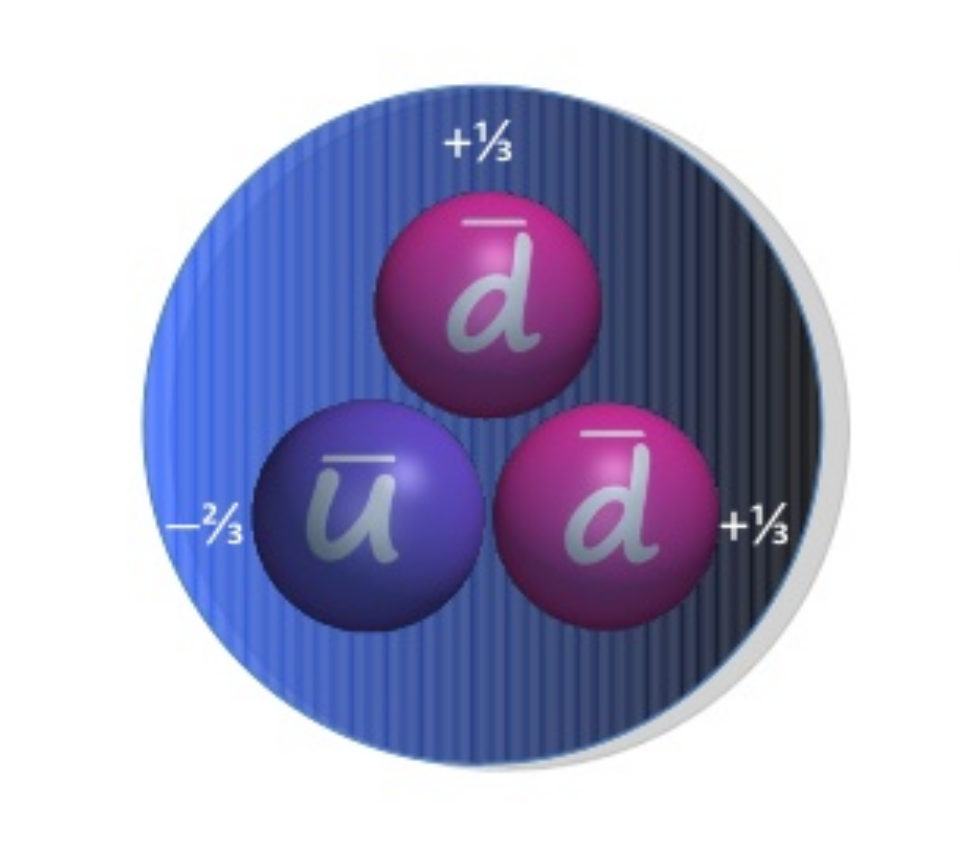
\includegraphics[width=0.3\textwidth]{Antineutron}
\end{figure}
\begin{itemize}
  \item the antineutron is a Bayron wich consits of 3 quarks.
  \item gets deteced in hadronic Calorimeters where the annihilation energy gets collected
\end{itemize}
% Today we know that the antineutron is a Bayron wich consits of 3 quarks. \\
% It gets deteced in hadronic Calorimeters. The techenique is basically the same as
% in the experiment, it annihilates and the energy gets collected.
\end{frame}

%------------------------------------------------
\begin{frame}
\frametitle{Questions?}
\end{frame}

%------------------------------------------------

%------------------------------------------------

%----------------------------------------------------------------------------------------

\end{document}
